\chapter{教程的实现代码在哪里获得}

本书的 \LaTeX{} 源文件与配套示例代码统一托管在作者的 Gitee 仓库中：

\begin{center}
\url{https://gitee.com/rabbitc999/STM32\_PROGRAM}
\end{center}

仓库主页如图~\ref{fig:gitee-home}~所示。

\begin{figure}[htbp]
\centering 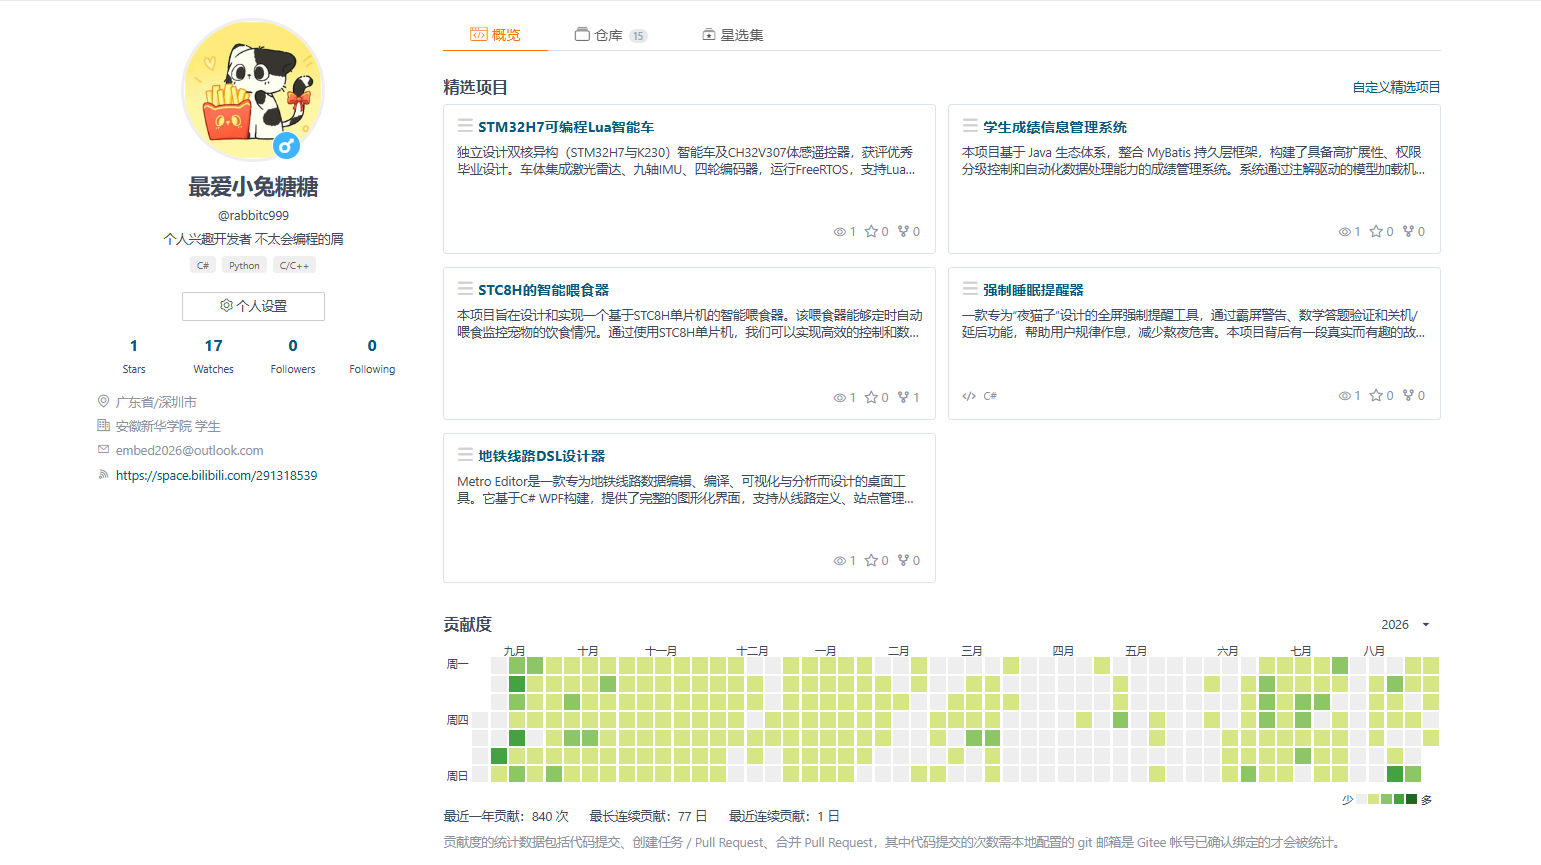
\includegraphics[width=\textwidth]{figure/Gitee.png} \caption{STM32\_PROGRAM 仓库主页} \label{fig:gitee-home}
\end{figure}

% ---------------------------------------------------------------------
\section{如何获取代码}

\subsection{方式一：Git 克隆（推荐）}

在安装了 Git 的电脑上执行：

\begin{lstlisting}
git clone https://gitee.com/rabbitc999/STM32_PROGRAM.git
\end{lstlisting}

克隆后可通过 \texttt{git pull} 获取后续更新。

\subsection{方式二：网页下载 ZIP}

如果不想安装 Git，也可以打开仓库主页，点击页面右上角的“克隆或下载”，选择“下载 ZIP”即可得到当前版本的完整压缩包。

% ---------------------------------------------------------------------
\section{仓库目录结构}

当前仓库主要包含以下几类内容：

\begin{itemize}
\item \texttt{Book/chapters/}：本书全部 \LaTeX{} 章节源码；
\item \texttt{Chapter-embed-basic/} $\sim$ \texttt{Chapter-memory-hardfault/}：按章节整理的示例代码，每章代码目录内部再按小节或功能拆分；
\item \texttt{Book/book.tex}：主文档，按顺序引入全部章节；
\item \texttt{AGENTS.md}：仓库代码规范，AI 协作开发时自动遵守；
\item \texttt{README.md} 与 \texttt{LICENSE}：仓库说明与开源协议。
\end{itemize}

其中：

\begin{itemize}
\item PC 上可直接编译的示例通常附带 \texttt{main.c} 与头文件，可使用 GCC 验证；
\item Keil 与 STM32CubeIDE 工程会保留完整的 \texttt{Project/Hardware/System} 目录；
\item 需要硬件环境的代码会在章节或 README 中标注“Untested，也称待实测”。
\end{itemize}

% ---------------------------------------------------------------------
\section{如何根据章节查找代码}

查找代码时建议按“章节主题”定位：

\begin{enumerate}
\item 先在仓库顶层找到与章节同名的 \texttt{Chapter-*} 目录；
\item 若代码目录名与章节小节名不一致，以目录内 \texttt{README.md} 或源码注释为准。
\end{enumerate}

% ---------------------------------------------------------------------
\section{代码协议与使用说明}

本教程的 \LaTeX{} 源文件与示例代码使用 GPL-3.0 协议开源。你可以学习、复制、修改和分发这些内容，但分发修改后的版本时，应同样遵循 GPL-3.0 的约束，并保留原作者版权声明。

使用代码时请注意：

\begin{itemize}
\item 示例代码以教学为目的，作者不保证其在所有硬件上直接可用；
\item 带“Untested”前缀的代码尚未由作者完成板级验证，运行前请先阅读目录说明；
\item 如发现代码缺陷、文档错误或希望交流技术问题，可在 Gitee 仓库提交 Issue。
\end{itemize}

% ---------------------------------------------------------------------
\section{结语}

这本书是作者在实验室、竞赛和毕业设计中积累经验的整理。如果仓库中的代码能帮助你完成一个课程设计、一次比赛或一个正式项目，那它就是有意义的。欢迎在学习和使用过程中提出意见，让这份教程和代码一起变得更好。
